% !TeX spellcheck = en_US
% !TeX TS-program = pdflatex
% !BIB TS-program = biblatex
\documentclass[11pt,a4paper]{article}
\usepackage{jheppub}

\pdfoutput=1
% to be `\input` in subfolders,
% ... therefore the path should be relative to subfolders.

\usepackage{iftex}
\ifPDFTeX
\else
	\usepackage[UTF8
		,heading=false
		,scheme=plain % English Document
	]{ctex}
\fi
%\ctexset{autoindent=true}
\usepackage{indentfirst}

\input{../.modules/basics/macros.tex}
\input{../.modules/preamble_base.tex}
\input{../.modules/preamble_beamer.tex}
\input{../.modules/basics/biblatex.tex}


%Misc
	\usepackage{lilyglyphs}
	\newcommand{\indicator}{$\text{\clefG}$}
	\newcommand{\indicatorInline}{$\text{\clefGInline}$}

\newcommand{\legacyReference}{{
%	\clearpage\par
%	\quad\clearpage
	\def{\midquote}{\textbf{PAST WORK, AS TEMPLATE}}
	\newparagraph
}}

% Settings
\counterwithout{equation}{section}
\mathtoolsset{showonlyrefs=false}
%\DeclareTextFontCommand{\textbf}{\sffamily}

% Spacing
\geometry{footnotesep=2\baselineskip} % pre footnote split
\setlength{\parskip}{.5\baselineskip}
\renewcommand{\baselinestretch}{1.15}


%% List
%	\setlist*{
%		listparindent=\parindent
%		,labelindent=\parindent
%		,parsep=\parskip
%		,itemsep=1.2\parskip
%	}


\addtobeamertemplate{navigation symbols}{}{%
    \usebeamerfont{footline}%
%    \usebeamercolor[fg]{footline}%
    \hspace{1em}%
    \large\insertframenumber/\inserttotalframenumber
}

\makeatletter
\setbeamertemplate{headline}
{%
    \begin{beamercolorbox}[wd=\paperwidth,colsep=1.5pt]{upper separation line head}
    \end{beamercolorbox}
    \begin{beamercolorbox}[wd=\paperwidth,ht=2.5ex,dp=1.125ex,%
      leftskip=.3cm,rightskip=.3cm plus1fil]{title in head/foot}
      \usebeamerfont{title in head/foot}\insertshorttitle
    \end{beamercolorbox}
    \begin{beamercolorbox}[wd=\paperwidth,ht=2.5ex,dp=1.125ex,%
      leftskip=.3cm,rightskip=.3cm plus1fil]{section in head/foot}
      \usebeamerfont{section in head/foot}%
      \ifbeamer@tree@showhooks
        \setbox\beamer@tempbox=\hbox{\insertsectionhead}%
        \ifdim\wd\beamer@tempbox>1pt%
          \hskip2pt\raise1.9pt\hbox{\vrule width0.4pt height1.875ex\vrule width 5pt height0.4pt}%
          \hskip1pt%
        \fi%
      \else%  
        \hskip6pt%
      \fi%
      \insertsectionhead
    \end{beamercolorbox}
% Code for subsections removed here
}
\makeatother

%% detailed ToC
\setcounter{tocdepth}{3}

\usepackage{xspace}
\newcommand{\TTbar}{\texorpdfstring{\ensuremath{T\bar{T}}}{TTbar}\xspace}
\newcommand{\ads}[1]{\text{AdS}\ensuremath{_{#1}}}
\newcommand{\cft}[1]{\text{CFT}\ensuremath{_{#1}}}

%%%%%%%%%%%%%%%%%%%%%%%%%%%%%%%%%%%%%%%%%%%%%%
%%%%%%%%%%%%%%%%%%%%%%%%%%%%%%%%%%%%%%%%%%%%%%

\title{Holographic duality beyond AdS/CFT}

%\author[a]{Wen-Xin Lai,}
\author[a]{Wei Song}
%\author[a]{and Fengjun Xu}

\affiliation[a]{Yau Mathematical Sciences Center, Tsinghua University, Beijing 100084, China}

%\emailAdd{laiwx19@mails.tsinghua.edu.cn, wsong2014@mail.tsinghua.edu.cn}

\abstract{
	Lecture notes for the Southeast Summer School on Strings and Stuff, 2021. 
}

\begin{document}
\maketitle
%\flushbottom
\setlength{\parskip}{.5\baselineskip}

\addtocounter{section}{-1}
\section{Introduction}
	
	Since the discovery of AdS/CFT duality \cite{Maldacena:1997re}, we have greatly furthered our understanding of quantum gravity in asymptotically AdS backgrounds. However, there are plenty of non-AdS geometries in our real worlds, including:
	\begin{itemize}%[noitemsep]
	\item The Kerr metric of a rotation black hole, \sidenote{which ... };
	\item The asymptotically flat / Minkowski spacetime, which well approximates our current universe at a smaller length (and time) scale;
	\item The asymptotically de Sitter spacetime, which well approximates our current (and future) universe at a larger length scale, and also during the period of inflation;
	\item The FRW metric (or more precisely, the Friedmann-Lemaître-Robertson-Walker \cite{Friedmann:1924bb,Lemaitre:1933gd,Robertson:1935zz,Walker:1937} metric), which describes the evolution of our homogeneous and isotropic universe from the big bang to \sidenote{its ...} ;
	\item and more ...
	\end{itemize}
	Much less is known about quantum gravity in these backgrounds. 
	
	
\section{Brief review of \ads{3}/\cft{2}}
	
\section{Bottom-up approach: %based on
			from asymptotic symmetry}
	
	
\section{Top-down approach: %in 
			from string theory}
	
	String theory is a self-consistent theory of quantum gravity. 
	
	The first example of a microscopic counting of black hole entropy, discovered by Strominger-Vafa \cite{Strominger:1996sh}, comes from the \mbox{D1-D5-$P$} system in string theory. 
	
	The first incarnation of holographic principle was realized by Maldacena \cite{Maldacena:1997re}, by a stack of D3 branes in type IIB string theory. 
	
\subsection{The \mbox{D1-D5-$P$} system and its IR limit}
\label{sect:d1-d5-p}
	
	Let us look at the \mbox{D1-D5-$P$} brane configuration in type IIB string theory. This is well-reviewed in \cite{David:2002wn}. This configuration allows for an open string description and a closed string description. 
	
	\begin{table}[!htbp]
	\centering%\small
	%\setlength{\tabcolsep}{3pt}
	%\begin{adjustwidth}{-2em}{-5em}
	\begin{tabularx}{.7\linewidth}{
		~C{1.5}| ^C{.3}| ^C{1.5}|
		^C{.3} *4{ | ^C{.3} }
	}
	\toprule
		\textsf{Geometry} &
		\multicolumn{2}{~c|}{%
			\setrowstyle{\sffamily}%
			$\mathbb{R}^{4,1}$%
		} &
		$S^1$ &
		\multicolumn{4}{^c}{
			$\mcal{M}_4 = T^4, \mrm{K3}$
		}
	\\ %\cline{2-3}
	\midrule
		\textsf{Direction}
		& 0 & 1, 2, 3, 4 & 5 & 6 & 7 & 8 & 9 \\
	\midrule
		$\mop{\#}\text{\small D5} = Q_5$ &
		$\times$ & &
		$\times$ & $\times$ & $\times$ & $\times$ & $\times$
	\\
		$\mop{\#}\text{\small D1} = Q_1$ &
		$\times$ & &
		$\times$ & & & &
	\\
		$P$ &
		$\times$ & &
		$\times$ & & & &
	\\
	\bottomrule
	\end{tabularx}
	\caption[Brane configuration of the D1-D5-$P$ system]{
		Brane configuration of the D1-D5-$P$ system. 
%	\\
		Here we are considering type IIB string theory on flat 6D spacetime, with a compactified $x^5 \in S^1$ direction, along with an internal $\mcal{M}_4$ manifold. 
		We use $\mquote{\times}$ to mark the directions $x^\mu$ that an object occupies. Here $\mu = 0,1,\cdots,9$.
	}
	\end{table}
	
	The D5 branes wrap the compact $\mcal{M}_4$, while the D1 branes are localized on $\mcal{M}_4$. Both the D1 and D5 branes extend along the fifth direction $x^5$, which is compactified to a circle $S^1$ with a large radius. 
	
	Open string excitations on the branes carry momentum and winding. Due to the large radius of $S^1$, we can focus on the momentum modes $P$ along $x^5 \in S^1$ and neglect the winding modes. On the other hand, we will neglect momentum modes along the $\mcal{M}_4$ directions, since $\mcal{M}_4$ is assumed to be compact and small. 
	
\subsubsection{Closed string picture: gravity on \ads{3} background}
	In the IR limit, type IIB string theory is described by the low energy effective action of type IIB supergravity. The field content and the action of type IIB supergravity are well reviewed in the literature; see e.g.\ Appendix H of \cite{Kiritsis:1997hj}. In particular, there is a pair of 2-form gauge potentials in type IIB supergravity. One of them is the NS-NS field $B_2$, and the other is the R-R field $C_2$. 
	The D1 branes are electrically charged under $C_2$, while the D5 branes are magnetically charged under $C_2$. 
	
	The bosonic part of the string frame action is then given by \needcites:
	\begin{gather}
		\frac{1}{16\pi G}
		\int \dd[10]{x} \sqrt{-g}
			\pqty{
				e^{-2\phi} \Big(
					R + 4\,(\nabla\phi)^2
					- \sidenote{\frac{1}{12}} H^2
				\Big)
				- \sidenote{\frac{1}{12}} F^2
			},
	\\
		H = \dd{B_2},\quad
		F = \dd{C_2}
	\end{gather}
	where $H$ and $F$ are the 3-form field strengths, $H^2 = H_{\mu\nu\rho} H^{\mu\nu\rho} \mathbin{\sidenote{\propto}} H\wedge \hstar H$\wx{}{convention for the coefficients?}, and similar for $F^2$. 
	After dimension reduction of the compact $\mcal{M}_4$, the equations of motion admit a \textit{black string} solution in 6D, where the metric is given by \needcites:
	\begin{gather}
	\begin{aligned}
		\dd{s}^2
		= {} & (f_1 f_5)^{-1/2} \pqty{
				-\dd{t}^2 + \dd{\phi}^2
				+ \frac{r_0^2}{r^2} \pqty{
					\cosh\sigma \dd{t}
					+ \sinh\sigma \dd{\phi}
				}^2
			} \\
		& {} + (f_1 f_5)^{+1/2} \pqty{
				\frac{\dd{r}^2}{1 - r_0^2 / r^2}
				+ r^2 \dd{\Omega_3^2}
			},
		\quad \phi \cong \phi + 2\pi R,
	\end{aligned}
	\\[1ex] \text{where}
	\quad f_1 = 1 + \frac{r_1^2}{r^2},
	\quad f_5 = 1 + \frac{r_5^2}{r^2}
	\end{gather}
	The parameters in this supergravity solution can be related to the brane construction as follows:
	\begin{itemize}
		\item $\phi \equiv x^5$ is the compactified $S^1$ direction along the D1 brane, normalized such that $\phi \cong \phi + 2\pi R$, where $R$ is the large radius of the $S^1$ circle. 
		
		Upon dimension reduction of the $\phi$ direction, this 6D black string solution will become a 5D black hole solution. In fact the resulting 5D black hole solution is precisely the Strominger-Vafa black hole \cite{Strominger:1996sh}, which serves as the first example of a microscopic counting of the black hole entropy. 
		
		\item $r_0$ marks the horizon of the black string, and it is related to the open string momentum $P$ attached to the branes: $P \propto r_0^2 \sinh 2\sigma$. 
		
		\item $r_1^2$ and $r_5^2$ are related to the charges $Q_1$ and $Q_5$. 
	\end{itemize}
	
	We further note that the above black string solution is asymptotically flat, consistent with our brane construction in string theory. On the other hand, if we zoom in to the near horizon region of this black string solution, we discover an $\ads{3}\times S^3$ geometry. This can be achieved by setting:
	\begin{equation}
		\ell^2 = r_1 r_5,
	\quad r\mapsto \lambda\ell r,
	\quad r_0\mapsto \lambda\ell r_0,
	\quad t\mapsto t\ell / \lambda,
	\quad \phi\mapsto \phi\ell / \lambda,
	\end{equation}
	where $\ell$ is the \ads{} radius, and now the $\phi$ coordinate is normalized such that $\phi \cong \phi + 2\pi$. 
	More specially,
	\begin{itemize}
	\item For extremal black string with $r_0 = 0$ and thus $P = 0$, the near horizon limit leads to the zero mass BTZ geometry, with an additional $S^3$ factor:
	\begin{equation}
		\dd{s}^2
		= \ell^2 \pqty{
			r^2 (-\dd{t}^2 + \dd{\phi}^2)
			+ \frac{\dd{r}^2}{r^2}
			+ \dd{\Omega_3^2}
		}
	\end{equation}
	
	\item For the near-extremal case with generic $r_0, \sigma$, the near horizon limit leads to the rotating BTZ geometry, again with an additional $S^3$ factor:
	\begin{equation}
		\dd{s}^2
		= \ell^2 \pqty{
			r^2 (-\dd{t}^2 + \dd{\phi}^2)
			+ \frac{\dd{r}^2}{r^2 - r_0^2}
			+ r_0^2 \pqty{
				\cosh\sigma \dd{t}
				+ \sinh\sigma \dd{\phi}
			}^2
			+ \dd{\Omega_3^2}
		}
	\end{equation}
	
	\end{itemize}
	
	It is convenient to define the left and right-moving temperature:
	\begin{equation}
		T_L = \frac{1}{2\pi}
			\frac{r_0\,e^\sigma}{\ell^2},
	\quad
		T_R = \frac{1}{2\pi}
			\frac{r_0\,e^{-\sigma}}{\ell^2}
	\end{equation}
	On the other hand, the Hawking temperature $T_H$ of this solution can be computed, and is given in terms of $T_L,T_R$ as follows:
	\begin{equation}
		\frac{2}{T_H}
		= \frac{1}{T_L}
		+ \frac{1}{T_R}
	\end{equation}
	
	\wx{Within the framework of string theory, one can understand the IR black string geometry as the result of ``integrating out'' the dynamics of the branes, which includes the open string excitations.}{accurate?} This process deforms the background geometry, and we end up with a closed string theory on the black string background. The near horizon limit brings us further to the IR fixed point, where the far region dynamics decouple and we are left with the \ads{3} geometry. 
	
	In other words, strings on $\ads{3}\times S^3\times \mcal{M}_4$ is understood as the \textit{closed string description} of the IR fixed point of the D1-D5-$P$ system. 
	
\subsubsection{Open string picture: worldvolume \cft{2} and the duality}
	
	On the other hand, we can consider the worldvolume theory of the brane construction. This provides the \textit{open string description} of the D1-D5-$P$ system. 
	
	After dimension reduction of the compact $\mcal{M}_4$, we have a $(1+1)$ dimensional QFT living on the D1-D5 branes. This is a supersymmetric gauge theory with $\mcal{N} = (4,4)$ supersymmetry. 
	Similar to our previous discussions, we can consider the IR limit of this system. It should flow to an IR fixed point, which is a $(1+1)$ dimensional superconformal field theory (S\cft{2}). 
	
	The central charge of this S\cft{2} can be read off from the field contents of the worldvolume theory: the number of bosonic fields is given by \needcites: 
	\begin{equation}
		4Q_1 Q_5
	\end{equation}
	and same for the fermions. The factor $Q_1 Q_5$ comes from the open string excitations between the D1 and D5 branes, while the factor of 4 comes from the fact that the D1 branes can move inside the D5 branes \wx{along the compact $\mcal{M}_4$ directions.}{is this language accurate?} In the end we have the central charge:
	\begin{equation}
		c = 1\times 4Q_1 Q_5
			+ \frac{1}{2}\times 4Q_1 Q_5
		= 6Q_1 Q_5
	\end{equation}
	
	We have thus discovered two equivalent descriptions of the D1-D5-$P$ system, summarized as follows:
	\begin{equation*}
	\begin{array}{ccc}
		\pqty{
			\ \begin{gathered}
				\text{Far-region dynamics} \\
				+ \\
				\text{Strings on $\ads{3}\times S^3\times \mcal{M}_4$}
			\end{gathered}\ %
		}
		&=&
		\pqty{
			\ \begin{gathered}
				\text{Far-region dynamics} \\
				+ \\
				\text{S\cft{2} with target $\mcal{M}_4$}
				\vphantom{S^3}
			\end{gathered}\ %
		}
	\\[6ex]
		\textit{Closed string picture}
		& &
		\textit{Open string picture}
	\end{array}
	\end{equation*}
	The far-region dynamics decouple on both sides, and we have the following proposal of an \ads{3}/\cft{2} duality \needcites:
	\begin{equation}
	\begin{aligned}
		&\text{Type IIB string theory on $\ads{3}\times S^3\times \mcal{M}_4$} \\
		{} = {}
		&\text{Marginal deformations of some $\mcal{N} = (4,4)$ S\cft{2} with target $\mcal{M}_4$}
	\end{aligned}
	\end{equation}
	Note that both sides of the duality includes a non-trivial moduli \needcites. \wx{In particular, the S\cft{2} on the right-hand side is proposed to be a \textit{symmetric product orbifold theory} \needcites, together with its exactly marginal deformations along the conformal manifold. }{elaborate?}
	
\subsection{Type IIB string theory with NS-NS flux}
	
	Due to its non-trivial coupling to the R-R field $C_2$, the D1-D5 system is difficult to deal with on the worldsheet, within the framework of the RNS (or NSR) formalism. This difficulty can be avoided by considering its S-dual, the NS1-NS5 system. 
	
	First let us recall the $\mrm{SL}(2,\mbb{Z})$ duality of type IIB string theory, reviewed in \S12 and \S14 of \cite{Polchinski:1998rr}. In particular, the strong-weak S-duality is one of the generators of the $\mrm{SL}(2,\mbb{Z})$ action. When acted on the field strengths $H = \dd{B_2}$ and $F = \dd{C_2}$, it's given by:
	\begin{gather}
		S\colon\ %
		\pqty{\begin{array}{c} H \\ F \end{array}}
		\ \longmapsto\ %
		\pqty{\begin{array}{cc}
			0 & 1 \\
			-1\hspace*{.2em} & 0
		\end{array}}
		\pqty{\begin{array}{c} H \\ F \end{array}}
		= \pqty{\begin{array}{c} F \\ -H \end{array}},
	\\[.5ex]
		H = \dd{B_2},\quad F = \dd{C_2} \nonumber
	\end{gather}
	We note that S-duality exchanges the field strengths $H$ and $F$. On the other hand, the D1-D5 system couples to $C_2$ (electrically for D1, and magnetically for D5), while the NS1-NS5 system couples to $B_2$. Therefore S-duality corresponds to a map:
	\begin{equation}
	S\colon\quad
	\begin{aligned}
		Q_5\ \,\text{D5 branes}
		\ \,&\longmapsto\ \,
		k = Q_5\ \,\text{NS5 branes} \\
		Q_1\ \,\text{D1 branes}
		\ \,&\longmapsto\ \,
		p = Q_1\ \,\text{NS1 branes} \\
	\end{aligned}
	\end{equation}
	
	We can then repeat the analysis in \S\ref{sect:d1-d5-p} and obtain a similar black string solution in 6D. By taking the near horizon limit, we further obtain an asymptotically \ads{3} geometry, namely the BTZ solutions as described in \S\ref{sect:d1-d5-p}, but now with NS-NS flux instead of R-R flux. In particular, for $P = 0$ we have the massless BTZ solution \needcites:
	\begin{gather}
		\dd{s}^2
		= k \pqty{
			\dd{\rho}^2
			+ e^{2\rho} \dd{\gamma} \dd{\bar{\gamma}}
		},
	\\
		B_2 = \frac{1}{2} B_{\mu\nu}
				\dd{x^\mu} \wedge \dd{x^\nu}
		= - \frac{k}{2}\,e^{2\rho}
				\dd{\gamma} \wedge \dd{\bar{\gamma}},
	\quad e^{2\Phi} = \frac{k}{p},
	\end{gather}
	where we note that there is a non-trivial $B$-field and a dilaton profile $\Phi$. 
	
	Why are we interested in this S-dual system? As we've mentioned before, unlike the original D1-D5 system, the NS1-NS5 system admits a worldsheet description as an RNS superstring theory. Therefore we have a well understood \textit{worldsheet} \cft{2} for the bulk string theory. Furthermore, based on this worldsheet \cft{2}, we are able to construct explicitly the \textit{dual} \cft{2} on the asymptotic boundary of the spacetime. This is sometimes referred to as the \textit{spacetime} \cft{2}. Therefore the NS1-NS5 system serves as a realization of \ads{3}/\cft{2} where both sides of the holographic duality are in some sense, under control. 
	
\section{Holographic Dualities Beyond \ads{3}/\cft{2}}

In the previous sections, we have laid down some basic aspects of \ads{3}/\cft{2} dualities in string theory. Starting from this section, we are going to introduce recent salient developments on holographic dualities beyond \ads{3}/\cft{2}. In particular, we will focus on $T\bar{T}$ deformation. This section is organized as follows:

\subsection{Top-Down Approach: Deformations of \ads{3}/\cft{2} in string theory}
In order to introduce deformations, we here remind the basic triangle among \ads{3}/\cft{2}. 



\begin{figure}[ht!]
\centering
 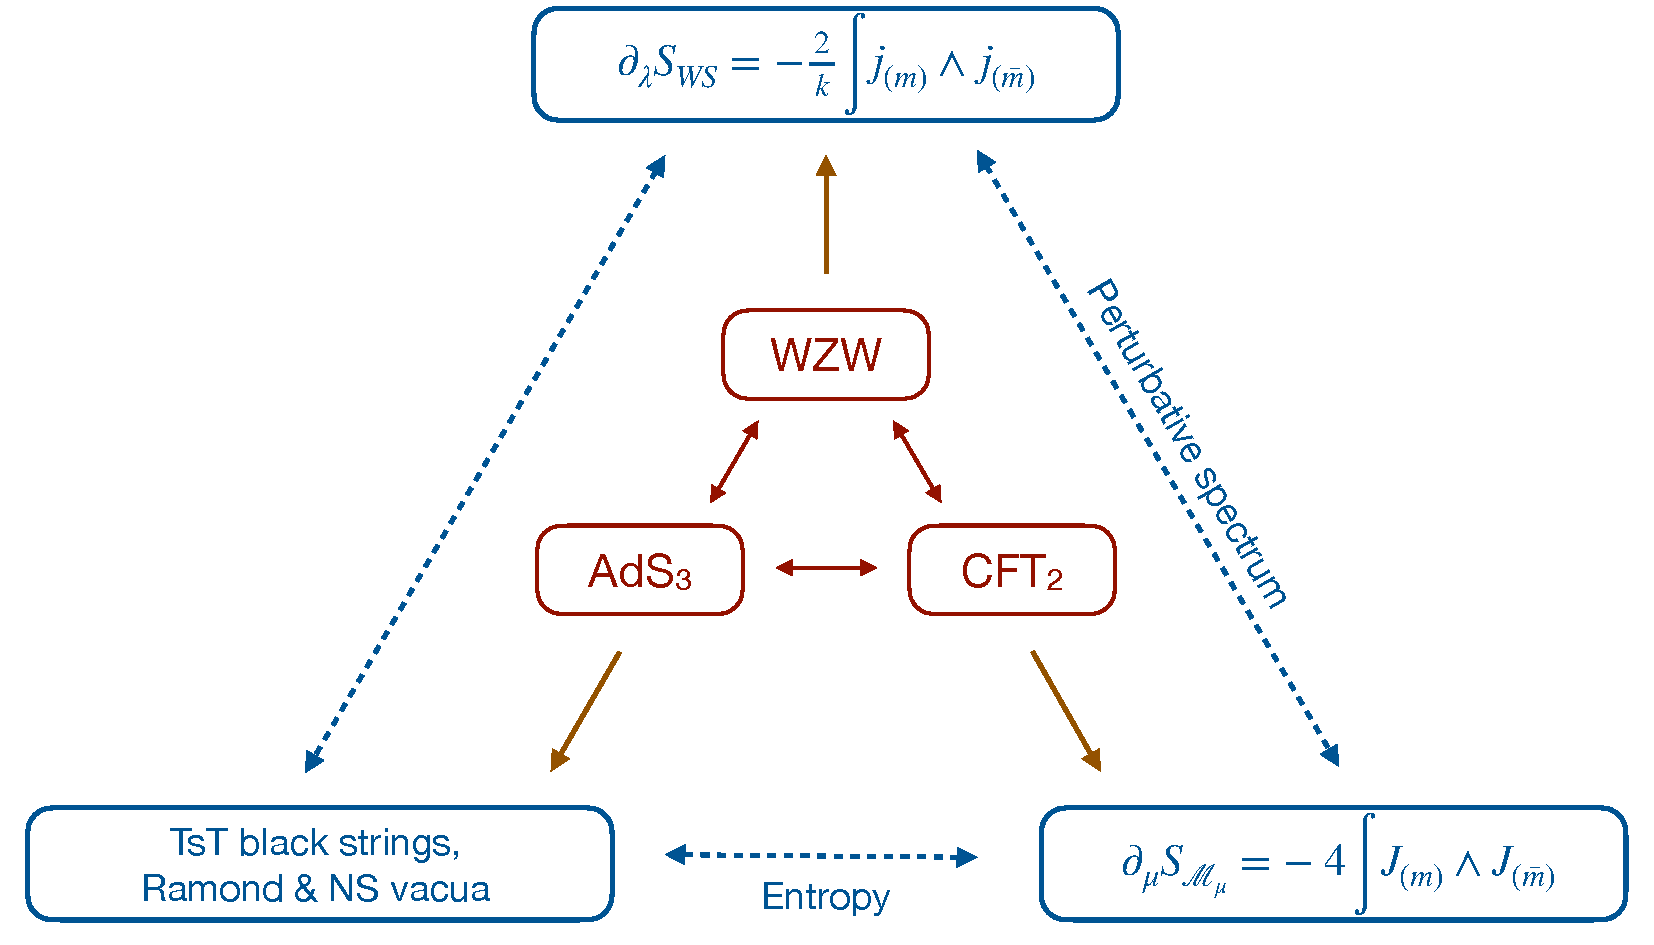
\includegraphics[scale=0.45]{img/diagram4}
\caption{The holographic correspondence between string theory on AdS$_3 \times M^7$ backgrounds and two-dimensional CFTs (inner triangle), and its relationship to the conjectured duality between TsT transformations of AdS$_3 \times M^7$ spacetimes, bi-current deformations of the worldsheet action, and single-trace irrelevant deformations of two-dimensional CFTs (outer triangle). 
Adapted from \cite{Apolo:2021wcn}}
\label{fig:triangle}
\end{figure}



\subsection{$T\bar{T}$ deformation}
In a Lorentzian invariant theory, the stress tensor $T^{\mu\nu}$ is conserved, i.e. $\partial_\mu T^{\mu\nu}=0$. One can define its determinant $\text{Det} T_{\mu\nu}$ as 
\begin{equation}
\begin{split}
    \mathcal O_{T\bar T}&:= \text{Det} T_{\mu\nu} \\
    &=T_{xx}T_{\bar x\bar x}-T_{x\bar x}T_{\bar{x} x} \\
    &=\text{Lim}_{x \rightarrow y} (T_{xx}(x)T_{\bar x\bar x}(y)-T_{x\bar x}(x)T_{\bar{x} x}(y) )+ \text{derivatives}
    \end{split}
\end{equation}
which is well-defined, and has 
\begin{equation}
    \langle n| \mathcal{O}_{T\bar T} |\rangle =\langle n| T |n\rangle \langle n|\bar T |n\rangle -\langle n| 
    \Theta|n\rangle \langle n|\bar{\Theta} |n\rangle
\end{equation}

The $T\bar T$ deformations can be described by deforming the CFT by an extra term 
\begin{equation}
     \frac{\p S_{\mathcal M_\mu}}{\p \mu} = \int d^2x \mathcal{O}_{T\bar T}
\end{equation}

where we have combine the 2d spacetime coordinate $(\phi, t)$ into  $x=\phi+t$ and $\bar{x}=\phi-t$.

When putting the deformed CFT on a cylinder, with $(x, \bar x) \sim (x+ 2\pi R, \bar x+2\pi R)$, one can then evaluate the energy spectra via invisited Burger's equation:
\begin{equation}
    \p E_n(R, \mu)= E_n(R, \mu) \p E(R, 0)+\frac 1{R} J_n^2(R)
\end{equation}

The spectrum 

  \eq{
  E(\mu) &= - \frac{ R}{2 \mu} \Bigg[ 1 - \sqrt{1 + \frac{4 \mu}{ R} E(0) + \frac{4 \mu^2}{ R^4} J(0)^2} \,\Bigg], \qquad J(\mu) = J(0), \label{ttbarspectrum}
  }
  %  
where $E = E_L + E_R$ and $J = R(E_L - E_R)$ denote the energy and angular momentum.  

Let us make some comments on the $T\bar T$ deformation:
$\bullet$ it is irrelevant, since the dimension of $\mu$ is $2>0$. 

$\bullet$ It is also solvable, which is the main reason why people are interested in studying them. 

$\bullet$ It can also be reformulated as coupling to random geometry, flat $JT$ gravity, (non-) critical strings. 

$\bullet$ The partition function after the deformation is still modular invariant. 

$\bullet$ The scattering amplitude can be shown as dressed by a phase factor. 

From the histroric viewpoint, 



It was conjectured in \cite{Apolo:2019zai} that performing the following TsT transformation on the string theory is holographically equivalent to deforming the seed of the dual symmetric orbifold,
\begin{equation}
\textrm{TsT}_{(X^m,X^{\bar m};\check\mu)} \quad\Longleftrightarrow\quad  \frac{\p S_{\mathcal M_\mu}}{\p \mu} = -4 \int J_{(m)} \wedge J_{(\bar{m})}, \label{conjecture}
\end{equation}
where $\textrm{TsT}_{(X^m,X^{\bar m};\check\mu)}$ denotes T-duality on  $X^m$, shift $ X^{\bar m} \to X^{\bar m} - 2\check\mu X^m$,  and T-duality on $ X^m$, $S_{\mathcal M_\mu}$ is the action of the deformed seed, $\mu$($\check\mu$) is the dimensionful(less) deformation parameter, and $J_{(m)}$, $J_{(\bar{m})}$ are the Noether currents generating translations along $X^m$, $X^{\bar m}$. It is interesting to note that from a purely worldsheet perspective, a TsT transformation is equivalent to a \emph{marginal} bi-current deformation of the worldsheet action, the latter of which can be shown to be equivalent to a gauged $(SL(2,R) \times U(1))/ U(1)$ WZW model~\cite{Apolo:2019zai}.


%%%%%%%%%%%%%%%%%%%%%%%%%%%%%%%%%%%%%%%%%%%%%%
%%%%%%%%%%%%%%%%%%%%%%%%%%%%%%%%%%%%%%%%%%%%%%

\pagebreak
\bibliographystyle{JHEP} 
\bibliography{beyondAdS.bib}

\end{document}

% vim: set ts=4 sw=4 sts=4 noexpandtab:
